
%%%%%%%%%%%%%%%%%%%%%%% file typeinst.tex %%%%%%%%%%%%%%%%%%%%%%%%%
%
% This is the LaTeX source for the instructions to authors using
% the LaTeX document class 'llncs.cls' for contributions to
% the Lecture Notes in Computer Sciences series.
% http://www.springer.com/lncs       Springer Heidelberg 2006/05/04
%
% It may be used as a template for your own input - copy it
% to a new file with a new name and use it as the basis
% for your article.
%
% NB: the document class 'llncs' has its own and detailed documentation, see
% ftp://ftp.springer.de/data/pubftp/pub/tex/latex/llncs/latex2e/llncsdoc.pdf
%
%%%%%%%%%%%%%%%%%%%%%%%%%%%%%%%%%%%%%%%%%%%%%%%%%%%%%%%%%%%%%%%%%%%


\documentclass[runningheads,a4paper]{llncs}

\usepackage{amssymb}
\setcounter{tocdepth}{3}
\usepackage{graphicx}
\usepackage{subfigure}
\usepackage{float}
\usepackage{alltt}
\usepackage{algorithm}
%\usepackage[sans]{dsfont}
%\usepackage{caption}

\usepackage{url}
\urldef{\mailsa}\path|{leonid.antsfeld, daniel.harabor,
toby.walsh}@nicta.com.au, adibotea@ie.ibm.com| \urldef{\mailsb}\path||
\urldef{\mailsc}\path||
\newcommand{\keywords}[1]{\par\addvspace\baselineskip
\noindent\keywordname\enspace\ignorespaces#1}

\begin{document}

\mainmatter  % start of an individual contribution

% first the title is needed
\title{Extracting Shortest Path using TRANSIT and CPDs in Video Game Maps}

% a short form should be given in case it is too long for the running head
%\titlerunning{Lecture Notes in Computer Science: Authors' Instructions}

% the name(s) of the author(s) follow(s) next
%
% NB: Chinese authors should write their first names(s) in front of
% their surnames. This ensures that the names appear correctly in
% the running heads and the author index.
%
\author{Leonid Antsfeld \and Daniel Harabor \and Adi  Botea  \and Toby Walsh}

\institute{
UNSW, Sydney NSW 2052 Australia\\
ANU, Canberra, ACT, 0200 Australia\\
NICTA, Kensington NSW 2052 Australia\\
IBM Research, Dublin, Ireland\\
\vspace{0.4cm}
\hspace{-0.4cm}
\mailsa\\
}


\maketitle

\section{Introduction}
We present a new algorithm for fast extraction of the shortest path in a grid video game maps, represned as grid networks.
The presented algorithm combines strength of two well know algorithms TRANSIT~\cite{bast06} and CPD~\cite{sanka05}.
The first one is a well established technique used for very fast shortest path distance (or travel time) queries in road networks.
The later is very efficient algorithm for fast path extraction in grid networks.

\section{Related work}

Most route planning methods rely on searching online.
On grid maps, a baseline approach uses A*~\cite{hart68} with 
the Manhattan heuristic, on 4-connected grid maps,
and the Octile heuristic on 8-connected maps.
These heuristics correspond to the true distance on a map with no obstacles.

Numerous enhancements to this baseline framework can broadly be grouped into
a few categories. Computing more informed heuristics is typically based on
pre-processing~\cite{goldberg05,bjornsson06,sturtevant09}.
Hierarchical abstraction replaces an original, flat search space with a
series of smaller searches~\cite{botea04,sturtevant05}.
Symmetry elimination can lead to strong prunning 
capabilities~\cite{harabor10,harabor11b}.

Real-time search without scrubbing
Competition entries.

Methods based on search can be relatively slow, as the number of 
nodes visited in a search is often much larger than the actual returned path.
Furthermore, the \emph{first-move lag}, which is the time needed before
obtaining at least one move, could be large as well, given that a first move
becomes available only after completing a search.

Transit and CPDs do not require a graph search process at runtime.
They pre-process and cache sufficient information to efficiently
answer queries on all-pairs shortest path data.

%Our approach fits here: optimality is required; move-by-move retrieval with low
%first-move lag; pre-processing is ok, memory is ok -- but we want to improve
%things.


\section{TRANSIT routing}\label{sec:transit}


The TRANSIT algorithm is based on a very simple intuition inspired from real-life navigation: when traveling
between two locations that are ``far away'' one must inevitably use some small set of edges that
are common to many shortest paths (highways are a natural example).
The endpoints of such edges constitute a set of so-called ``transit nodes'' for which the algorithm is named.
TRANSIT proceeds in two phases: (i) an offline precomputation phase and (ii) an online query phase.

\subsection {Offline Precomputation Phase}\label{sub:precomputation}
TRANSIT's offline precomputation phase consists of two main steps. At the first step we identify the aforesaid transit nodes
and in the second step we build a database of exact distances between every node and its associated transit nodes, as well as between all transit nodes.
We will describe each step in turn.

\subsubsection{Identifying Transit Nodes}\label{sub:determine}
TRANSIT starts by dividing an input map into a grid of equal-sized cells~
\footnote{ This grid is distinct from the one representing the input map.}.
To achieve this TRANSIT computes a bounding box for the entire map and divides this box
into $g \times g$ equal-size cells. Let $C$ denote such a cell. Further, let $I$ (Inner) and $O$ (Outer)
be squares having $C$ in the center, as depicted in Fig. \ref{fig:example} below.

\begin{figure}[H]
\centering
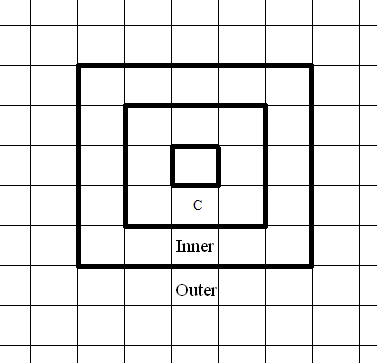
\includegraphics[height=5cm]{transit_example3.PNG}
\caption{Example of the TRANSIT grid; also cells and inner and outer squares. }
\label{fig:example}
\end{figure}

The size of the squares $C$, $I$ and $O$ can be arbitrary without compromising correctness. Their exact
values however will directly impact factors such as TRANSIT's preprocessing time, storage requirements and
online query times. In ~\cite{leon_daniel} we discuss how those parameters can be tuned and the tradeoff
between precomputation time, memory requirements and finally the query time.

In what follows we will compute shortest paths between nodes that resides on border of $C$ and $O$ and choose as
transit nodes one of the endpoints of the edges that cross the border of $I$. More precisely,
let $V_C$ be set of nodes as follows: for every link that has one of its endpoints inside $C$ and the other outside $C$,
$V_C$ will contain the endpoint inside $C$. Similarly, define $V_{I}$ and $V_{O}$ by considering links that cross $I$ and $O$ accordingly.
Now, the set of transit nodes for the cell $C$ is the set of nodes $v \in V_{I}$ with the property that there exists a shortest path from
some node in $V_C$ to some node in $V_{O}$ which passes through $v$. We associate every node inside $C$ with the
set of transit nodes of $C$. Next, we iterate over all cells and similarly identify transit nodes for every other cell.

\subsubsection{Computation and Storage of Distances}
\label{sub:precompute}
Once we have identified all transit nodes, we store for every node on the map, the shortest distance
from this node to all its associated transit nodes.  Recall from the previous section that every
such node $v \in V$ is associated with the set of transit nodes that were found for its cell.  In
addition we also compute and store the shortest distance from each transit node to every other
transit node.  In an undirected map it is enough to compute and store costs only in one direction.

\subsection {Local Search Radius}
\label{sub:local_radius}
TRANSIT distinguishes between two types of queries: local and global.  Two nodes for which
horizontal or vertical distance (as measured in number of cells) is greater than some \emph{local search
radius} are considered to be "far away" and the query between them is global.  We define
local search radius to be equal to the size of the inner square $I$ plus the distance from $I$ to the
outer square $O$.
This definition guarantees that for each global query two important conditions are satisfied:
 (i) the start node $src$ and destination node $dst$ are not inside the outer squares of each other
(ii) their corresponding inner squares do not overlap.
Both conditions are necessary to ensure the TRANSIT algorithm is correct and optimal.

\subsection{Online Query Phase}\label{sub:query}
For every global query from $src$ to $dst$ we fetch the transit nodes associated with cells containing
$src$ and $dst$ and choose those two that will give us a minimal cost of the combined three subpaths:
$src \rightsquigarrow T_{src}$, $T_{src} \rightsquigarrow T_{dst}$, $T_{dst} \rightsquigarrow dst$.
For all local queries the inventors of TRANSIT suggested to apply any efficient search algorithm; A* for example \cite{bast06}.
In what follows we will present a new, more efficient technique, using CPDs for dealing with local queries.

\subsection{Shortest Path Extraction}\label{sub:path_extraction}
Until now, not much work have been done on efficient path extraction using TRANSIT precomputed databases.
The intuitive and somewhat naive way would be performing a series of repeated distance queries of TRANSIT.
In the original paper the authors suggested first finding the next adjacent node to the source on the shortest path
and then iteratively applying TRANSIT query from that node to extract the full path ~\cite{bast06}.
An immediate improvement of this approach would be that we can store the next node of every precomputed
shortest path, rather than search for it.  Than we apply similar technique, by simply fetching the next adjacent node of the shortest path.
More sophisticated improvement can be achieved by observing that actually the transit node associated with destination, $T_{dst}$,
is not changing for all the sequential queries. Therefore we can exploit this fact and save time for looking for $T_{dst}$ every iteration, but 
rather reuse it.
In section ~\ref{sec:transit_cpd} we will present in details a novel, more efficient approach for the shortest path path extraction,
which is a main contribution of this paper.

\section{Compressed Path Databases}

Compressed Path Databases (CPDs)~\cite{botea11,DBLP:conf/socs/Botea12} are
all-pairs shortest path (APSP) data in a compressed form.
A fast retrieval of individual moves contained in a solution path, and the
optimality of moves are key strengths of CPDs. The so-called \emph{first-move
lag}, which is the time needed until a first move can be provided, is low,
since fetching one move is independent of subsequent moves on a path. 
Such strengths come at the price of a
significant pre-processing time, needed to compute all-pairs shortest path data,
and a significant amount of memory needed to store the pre-processing results.

Given a map, the pre-processing is done offline, being amortized over
all queries on that map. As shown later in this section, pre-processing can
easily be paralellized, since it consists of a series of independent
iterations. Yet, the pre-processing time can be critical, for instance in
cases such as a dynamic environment, which would require a re-computation of a CPD.

Despite the ability of CPDs to compress APSP data by hundreds of
times without any information loss,
their size can sometimes be a performance bottleneck,
depending on the map size, the topology, and the amount of RAM available.
Further reducing the memory needs and the pre-processing time are main
contributions of this work.

A detailed overview of computing and using CPDs is beyond the scope of this
paper, especially since, in our approach, the CPD method can be used as a
blackbox tool. For a detailed description, we point the reader to the original
publications~\cite{botea11,DBLP:conf/socs/Botea12}.

% In the pre-processing phase, APSP data are computed with a series of independent
% iterations. There is one iteration for each node $n$ on the map.
% An invocation of the Dijkstra algorithm allows computing an optimal move
% $\mbox{move}(n,t)$ from $n$ towards any reachable target $t$ on the map. The
% result is two-dimentional table $T(n)$, called a first-move table, with the same
% number of rows and columns as the map.
% At cell $(c,r)$, it contains $\mbox{move}(n,t)$, where $t$ is the node graph
% with column $c$ and row $r$.
% 
% As a second step of an iteration, a first-move table is compressed 



\section{TRANSIT with CPD}\label{sec:transit_cpd}
The basic idea of our approach is to break a long shortest path (i.e. $src \rightsquigarrow dst$ is a global query)  
to number of shorter, local subpaths: $$src=T_0 \rightsquigarrow T_1 \rightsquigarrow T_2 ...\rightsquigarrow... T_{k-1} \rightsquigarrow T_{k}=dst.$$
Then we build our $src \rightsquigarrow dst$ path by sequentially extracting local subpaths $T_i \rightsquigarrow T_{i+1}, i=0...k$ from partially precomputed CPDs.
Since CPDs queries are only local, it means that we need to precompute CPDs only for pairs of nodes which are within local search radius of each other.
This is a major saving in both precomputation time and memory requirements of CPD.
\\
We start with invoking the basic TRANSIT query. From section~\ref{sub:query} we remember that every global shortest path,
(i.e. it is longer than a local search radius) is of a form: $src \rightsquigarrow T_{src} \rightsquigarrow T_{dst} \rightsquigarrow dst$. 
By definition, subpaths $src \rightsquigarrow T_{src}$ is local (i.e. no longer than a local search radius)
therefore we are applying CPDs query to extract shortest path from $src$ to $T_{src}$. Next, if $T_{src} \rightsquigarrow dst$ is a local query,
we extract this subpath from CPDs as before and we are done. 
If $T_{src} \rightsquigarrow dst$ is a global query, then we will repeat the above procedure 
but this time using $T_{src}$ as our new $srs$. We can improve this even more, by noticing that when running sequentials quires of TRANSIT $T_{dst}$
and the distance from $T_{dst}$ to $dst$ are not changing. We can exploit this fact, by reusing $T_{dst}$. This will speed up the time complexity 
of subsequent TRANSIT queries from quadratic to linear by the number of the transit nodes.
Below we presnet the pseudocode of the described algorithm. For clarity of the idea we present the simplified version here.
\begin{algorithm}
\begin{alltt}

   (\(T\sb{src}, T\sb{dst}) \leftarrow \) TRANSIT.query(src, dst);
   CPD.getShortestPath(src, \(T\sb{src}\));  
   while (true)                       
   \{
      if (isLocalQuery(\(T\sb{src}, dst\)) == true)
      \{
         CPD.getShortestPath(\(T\sb{src}, dst\));
         break;
      \}
      (\(\bar{T}\sb{src}, \bar{T}\sb{dst}) \leftarrow \) TRANSIT.query(\(T\sb{src}, dst\));
      CPD.getShortestPath(\(T\sb{src}, \bar{T}\sb{src}\));
      \(T\sb{src} := \bar{T}\sb{src}\)  
   \}

\end{alltt}
\caption{Pseudo code for extracting the shortest path between \textit{src} and \textit{dst}} \label{alg:transit_cpd_pseudo}
\end{algorithm}

One of the advantages of this approach over the techniques mentioned in section ~\ref{sub:path_extraction} is that we advance from $src$ to $dst$ by "chunks"
of local subpaths, rather than by single link. In addition for every such "chunk" we exploit the strength of the CPD algorithm that is
very efficient for local shortest path queries. In the next section we will present a comparative analysis of this algorithm.

\section{Experimental setup}

\section{Results}

\section{Discussion}

\section{Conclusions}

bla bla~\cite{bast06}

\bibliographystyle{plain}
\bibliography{references}

\end{document}

